\section{Introdu{\c c}{\~a}o}
\label{sec:intro}
Um modelo eficiente de fluxo de trabalho e versionamento {\'e} muito importante para o bom desenvolvimento de um projeto de software, j{\'a} que um dos principais problemas conhecidos do desenvolvimento e manuten{\c c}{\~a}o de software {\'e} o fen{\^o}meno denominado pelo termo "dependency hell". Este fen{\^o}meno acontece devido aos projetos de software possu{\'i}rem depend{\^e}ncias diretas e transitivas (depend{\^e}ncias de depend{\^e}ncias) que na verdade, nada mais s{\~a}o do que outros componentes de softwares que evoluem de forma independente cada qual com seu ciclo de vida e sua equipe. Assim sendo, quanto mais depend{\^e}ncias um projeto possui, maior a probabilidade de ocorrerem conflitos entre elas.

Vincent Driessen prop{\^o}s um modelo eficiente de fluxo de trabalho chamado Git-Flow ~\cite{gitflow} por{\'e}m, tal modelo pode vir a ser complexo para equipes pouco entrosadas ou pouco experientes ao trabalhar com sistema de controle de vers{\~o}es distribu{\'i}do dado uma quantidade grande de branches que tal modelo prop{\~o}e. No modelo de Driessen, temos um branch para desenvolvimento do projeto, outros tempor{\'a}rios para cada nova funcionalidade desenvolvida, um branch para release, o branch master (principal) que {\'e} usado somente para manter as vers{\~o}es finais com suas respectivas tags e um branch somente para os hotfixes.
Por meio deste artigo proponho uma maneira mais simples de fluxo de trabalho que acredito funcionar melhor em tais cen{\'a}rios e com bom aproveitamento de projetos desenvolvidos sob metodologia SCRUM~\cite{scrum} e implementados utilizando a ferramenta de gerenciamento de ciclo de vida Maven. Uma outra boa premissa tamb{\'e}m {\'e} o uso de um modelo de versionamento sugerido pela equipe de Tom Preston-Werner, cofundador do GitHub chamado Versionamento Sem{\^a}ntico~\cite{semver} sob a licen{\c c}a Creative Commons como pode ser visto na figura \ref{fig:modelogitflow}

\begin{figure}[h!]
\centering
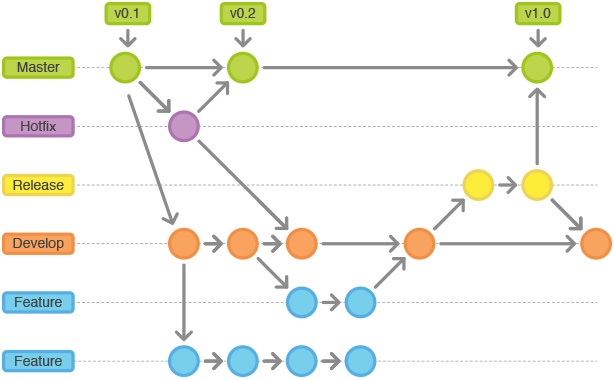
\includegraphics[width=0.7\linewidth]{img/modelo_gitflow}
\caption[Modelo de Branching GitFlow]{Modelo de branching proposto por Vincent Driessen e usado no GitFlow}
\label{fig:modelogitflow}
\end{figure}

O Versionamento Sem{\^a}ntico padroniza a nomenclatura de versionamento de c{\'o}digo utilizando no m{\'i}nimo tr{\^e}s conjuntos de n{\'u}meros onde a vers{\~a}o do projeto {\'e} composto pela "vers{\~a}o maior"."vers{\~a}o menor"."vers{\~a}o de corre{\c c}{\~a}o", sendo que a vers{\~a}o maior {\'e} incrementada quando se tem mudan{\c c}as incompat{\'i}veis na API, a vers{\~a}o menor quando s{\~a}o adicionadas funcionalidades mantendo-se a compatibilidade da API e a vers{\~a}o de corre{\c c}{\~a}o para corre{\c c}{\~a}o de defeitos somente. Classificadores tamb{\'e}m podem ser aplicados ap{\'o}s a vers{\~a}o de corre{\c c}{\~a}o, dentre outros detalhes da nomenclatura presente em sua especifica{\c c}{\~a}o.
\\\\
Por exemplo:
\\\\
Projeto \textbf{FrameworkTeste} na vers{\~a}o:\textbf{ 1.2.3-SNAPSHOT} desenvolvido sob metodologia SCRUM:
\\\\
Assim sendo, podemos condiderar:
\\\\
\textbf{Vers{\~a}o Maior:} 1 - Primeira especifica{\c c}{\~a}o da API.\\
\textbf{Vers{\~a}o Menor:} 2 - Segundo conjunto de funcionalidades (muitas vezes associadas à segunda Sprint).\\
\textbf{Vers{\~a}o de Corre{\c c}{\~a}o:} 3 - Esta vers{\~a}o geralmente {\'e} incrementada v{\'a}rias vezes dentro de uma mesma Sprint).\\

No modelo proposto, sugiro o Git como refer{\^e}ncia de sistema de controle de versões dado o seu funcionamento distribu{\'i}do, simplicidade de altern{\^a}ncia entre diferentes branches e facilidade de reintegra{\c c}{\~a}o de c{\'o}digo (merge) e ser{\'a} usado como refer{\^e}ncia para este artigo por{\'e}m pode ser aplicado em qualquer SCM (Source Control Management). Utilizaremos tamb{\'e}m os classificadores (sufixos) adotados pelo Maven para diferenciar o projeto em estado de desenvolvimento (sufixo \textbf{-SNAPSHOT}) e estado de produto final (sem sufixo).
